\documentclass{report}
\usepackage{amsmath, amssymb, amsthm}
\usepackage{geometry}
\geometry{a4paper, margin=0.8in}
\usepackage{float}
\usepackage{tikz}
\usetikzlibrary{calc, decorations.pathreplacing}
\usepackage{pgfplots}
\pgfplotsset{compat=1.18}
\usepackage{xcolor}
\usepackage{tcolorbox}
\tcbuselibrary{theorems}
\usepackage{eurosym}
\usepackage{fancyhdr}
\usepackage{booktabs}

\begin{document}

\pagestyle{fancy}
\fancyhf{}
\rhead{Report 2 \;|\; Stochastic Methods for Finance \;|\; \thepage}
\renewcommand{\headrulewidth}{0.4pt}
\setlength{\headheight}{14pt}
\thispagestyle{plain} % Toglie l'header solo dalla pagina corrente (la prima)
% --- HEADER PROFESSIONALE ---
\begin{flushleft}
    {\large \textbf{Stochastic Methods for Finance - Report 2}} \\
    \textit{Implicit Dividend and Discount Factor Extraction} \\
    \rule{\textwidth}{0.4pt} \\ % Linea orizzontale sottile
    \textbf{Author:} Davide Quartucci \hfill \textbf{Date:} March 22, 2026 \\
    \textbf{Underlying:} EURO STOXX 50 (OESX) \hfill \textbf{Spot Price:} 5,501.28 pts \\
\end{flushleft}

% --- (Il tocco di classe) ---
\begin{center}
    \fcolorbox{black}{gray!10}{
        \begin{minipage}{0.95\textwidth}
            \small \textit{Every step implementation can be checked in the provided file:} \texttt{Report2\_Quartucci\_Davide.xlsx}
        \end{minipage}
    }
\end{center}

\section{Asset Selection and Market Data}
For this analysis, the EURO STOXX 50 index was selected as the underlying asset. The choice is justified by the high liquidity of its option chain and the European style of the contracts, perfect for applying the Put-Call Parity.

\section{Methodology}
The report follows a two-step quantitative approach to extract market-implied parameters.

\subsection{Discount Factor Estimation (Box Spread)}
To ensure an arbitrage-free discount factor $D(0,T)$, a Box Spread strategy was employed using two different strikes, $K_1$ and $K_2$. The discount factor is derived from the mid-prices of the respective Calls ($C$) and Puts ($P$):
\begin{equation}
D(0,T) = \frac{[C(K_1) - C(K_2)] + [P(K_2) - P(K_1)]}{K_2 - K_1}
\end{equation}
This method allows for a robust estimation of the present value of 1 unit of the index at maturity $T$ without requiring explicit knowledge of the risk-free rate.

\subsection{Implied Dividend Extraction (Put-Call Parity)}
The implied dividend, expressed as a present value ($PV_{div}$), is extracted using the Put-Call Parity relationship applied to At-The-Money (ATM) options ($K_{ATM}$):
\begin{equation}
C(K_{ATM}) - P(K_{ATM}) = D(0,T) \cdot (F_0(T) - K_{ATM})
\end{equation}
First, the Implied Forward price $F_0(T)$ is isolated:
\begin{equation}
F_0(T) = \frac{C(K_{ATM}) - P(K_{ATM})}{D(0,T)} + K_{ATM}
\end{equation}
Then, the present value of dividends is calculated by comparing the spot price with the discounted forward:
\begin{equation}
PV_{div} = S_0 - [F_0(T) \cdot D(0,T)]
\end{equation}

\section{Data Integrity and Strike Selection}
To maintain the integrity of the results, strike selection was adjusted based on market liquidity for each maturity. 
\begin{itemize}
    \item For the 1-month, 3-month, and 1-year maturities, a wide Box Spread was used to capture a broad market consensus.
    \item For the 6-month maturity, the Box Spread was lower. This adjustment was necessary because the available strikes were not sufficiently liquid.
\end{itemize}

\section{Results: Dividend Term Structure}
The following table summarizes the results obtained for the four analyzed maturities:

\begin{table}[h]
\centering
\begin{tabular}{lcccc}
\toprule
\textbf{Maturity} & \textbf{T (days)} & \textbf{Discount Factor} & \textbf{Implied Forward} & \textbf{Implied Div (pts)} \\
\midrule
17/04/26 (1m) & 26  & 0.9968 & 5,497.09 & 21.53 \\
19/06/26 (3m) & 89  & 0.9932 & 5,437.57 & 100.93 \\
18/09/26 (6m) & 180 & 0.9870 & 5,461.80 & 110.48 \\
19/03/27 (1y) & 362 & 0.9730 & 5,507.50 & 142.48 \\
\bottomrule
\end{tabular}
\caption{Summary of implied parameters and dividend term structure.}
\end{table}

\begin{figure}[h]
    \centering
    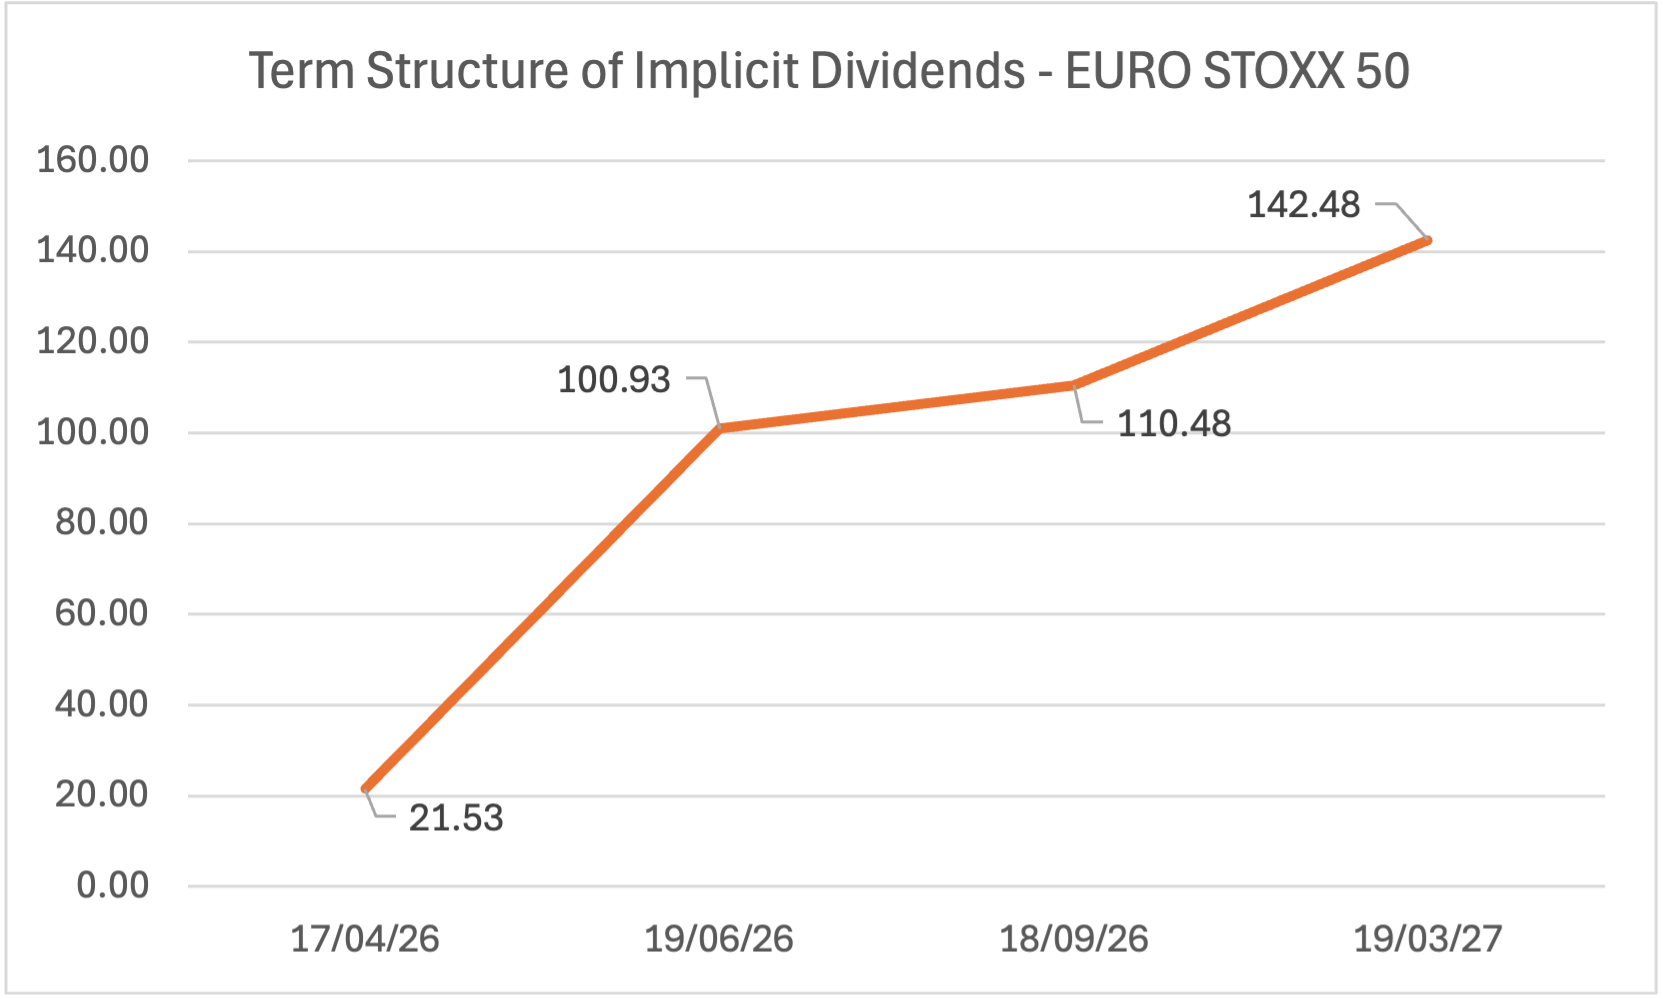
\includegraphics[width=0.8\textwidth]{Picture1.png}
    \caption{Term Structure of Implied Dividends.}
\end{figure}

\section{Analysis and Conclusion}
The derived dividend term structure exhibits a clear seasonal pattern typical of the European equity market. The significant jump in the present value of dividends between April (21.53 pts) and June (100.93 pts) reflects the "dividend season" concentrated in May, when major Euro Stoxx 50 constituents pay their annual coupons. 

\vspace{0.1cm}

The subsequent gradual increase towards the 1-year maturity (142.48 pts) confirms the cumulative nature of the distributions. The results demonstrate that the methodology of using Box Spreads and Put-Call Parity is highly effective for extracting market expectations from option prices, provided that data points are filtered for liquidity and arbitrage consistency.

\end{document}